\documentclass[letterpaper,12pt]{article}
\usepackage[spanish]{babel}
\spanishdecimal{.}
\usepackage[utf8]{inputenc}
\usepackage{graphicx}
\usepackage[top=2.5cm, bottom=2.5cm, left=2.5cm, right=2.5cm]{geometry}
\usepackage{hyperref}
\usepackage{amssymb}
\usepackage{gensymb}

\title{Práctica 3 \\ Transformaciones Homogéneas}
\author{Robots Bípedos Autónomos}
\date{Facultad de Ingeniería, UNAM}


\begin{document}
\renewcommand{\tablename}{Tabla}
\maketitle
\section*{Objetivos}
\begin{itemize}
\item Familiarizar al alumno con el concepto de Transformación Homogénea.
\item Aprender a utilizar el paquete \texttt{tf} para el manejo de transformaciones homogéneas.
\item Familiarizar al alumno con los archivos \texttt{urdf} para descripción de cadenas cinemáticas.
\end{itemize}

\section{Introducción}
\subsection{Movimiento rígido}
Para entender el movimiento en los robots bípedos, es necesario comprender primero los conceptos de movimiento rígido y transformación homogénea. Un movimiento rígido es una combinación de una posición y una orientación, es decir es un par ordenado $(d,R)$, donde $d\in \mathbb{R}^3$ y $R\in SO(3)$.

El conjunto $SO(3)$ se refiere al conjunto de matrices ortogonales de orden 3 (del inglés \textit{Special Orthogonal}). Las matrices del conjunto $SO(n)$ tienen varias propiedades especiales como el hecho de que su inversa es igual a su transpuesta, todos sus renglones y columnas son de magnitud 1 y ortogonales entre sí y que su determinante es siempre 1 (esto último si estas representan rotaciones de sistemas dextrógiros).

Entonces, un movimiento rígido es una combinación de una posición y una orientación. Estos movimientos también pueden ser usados para representar la Transformación de un sistema coordenado a otro, es decir, el par $(d, R)$ puede representar una rotación y una traslación. Es importante mencionar que, aunque la rotación $R$ puede darse sobre cualquier eje, en general siempre se manejan rotaciones sobre alguno de los ejes coordenados, por lo que $R$, en general, tiene alguna de las siguientes formas:
\[R_{x,\theta} = \left[
    \begin{tabular}{ccc}
      1 & 0 & 0\\
      0 & $\cos \theta$ & $-\sin \theta$\\
      0 & $\sin \theta$ & $\cos \theta$
    \end{tabular}
  \right]\qquad
  R_{y,\theta} = \left[
    \begin{tabular}{ccc}
      $\cos\theta$ & 0 & $\sin\theta$\\
      0 & 1 & 0\\
      $-\sin\theta$ & 0 & $\cos\theta$
    \end{tabular}
  \right]
\]
\[R_{z,\theta} = \left[
    \begin{tabular}{ccc}
      $\cos \theta$ & $-\sin \theta$ & 0\\
      $\sin \theta$ & $\cos \theta$  & 0\\
      0 & 0 & 1
    \end{tabular}
  \right]\]

\subsection{Transformaciones homogéneas}
Una transformación homogénea es la representación matricial de un movimiento rígido, es decir, es una matriz que representa una rotación más una traslación. Si la traslación está data por el vector $d=[d_x\;d_y\;d_z]^T$ y la rotación por la matriz $R_{k,\theta}\in SO(3)$, entonces la transformación homogénea $H$ que representa este movimiento es
\[H = \left[\begin{tabular}{cc}
    $R_{k,\theta}$ & $d$\\
    0 & 1
  \end{tabular}\right]\]
La matriz que representa la transformación inversa, es decir, el movimiento rígido opuesto, está dada por
\[H^{-1} = \left[\begin{tabular}{cc}
    $R^T$ & $-R^Td$\\
    0 & 1
  \end{tabular}\right]\]

Las transformaciones homogéneas generalmente se utilizan para representar la rotación y traslación de un sistema con respecto a otro. Si se tienen las coordenadas de un punto $p$ expresadas con respecto a un sistema $O_2$ y se desea obtener las coordenadas del mismo punto $p$ pero con respecto a otro sistema $O_1$, lo que se requiere es la rotación y traslación necesarias para llegar del sistema $O_1$ al sistema $O_2$.

Considere la figura \ref{fig:example}. Esta figura muestra a un robot humanoide que ha determinado, mediante su sistema de visión, la posición de una pelota. El sistema de visión obtuvo que las coordenadas de la pelota son $p = [p_x\;p_y\;p_z]^T = [1.2\;0\;-0.15]^T$ con respecto al sistema coordenado de la cámara $O_c$. Se desea obtener la posición de la pelota con respecto al centro de los pies del robot $O_r$. Se sabe que la posición del centro de la cámara está en el punto $d =[d_x\;d_y\;d_z]^T =[0.05\;0\;0.6]^T$ con respecto a $O_r$ y que el robot está volteando hacia abajo un ángulo de 30\degree, es decir, el sistema $O_c$ está rotado con respecto a $O_r$ un ángulo $\theta=\pi / 6$ sobre el eje $Y$.

\begin{figure}
  \centering
  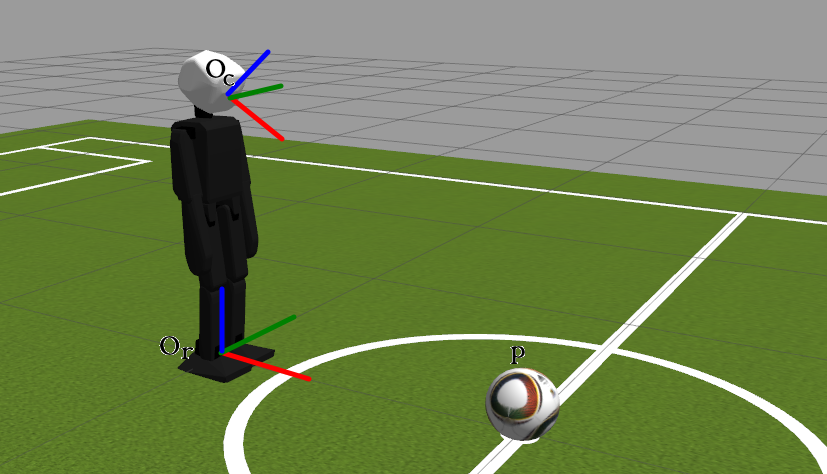
\includegraphics[width=0.6\textwidth]{example.png}
  \caption{Ejemplo de aplicación de las transformaciones homogéneas.}
  \label{fig:example}
\end{figure}

Para calcular la posición de la pelota con respecto a $O_r$ se construye la transformación homogénea:
\begin{equation}T_c^r = \left[\
  \begin{tabular}{cccc}
      $\cos\theta$ & 0 & $\sin\theta$ & $d_x$\\
      0 & 1 & 0 & $d_y$\\
      $-\sin\theta$ & 0 & $\cos\theta$ & $d_z$\\
      0 & 0 & 0 & 1
  \end{tabular}\right]
\end{equation}
La posición de la pelota se puede calcular como
\label{eq:transform}
\begin{equation}
  p_r =\left[\begin{tabular}{c}$p_{rx}$\\$p_{ry}$\\$p_{rz}$\\1\end{tabular}\right]
= \left[\
  \begin{tabular}{cccc}
      $\cos\theta$ & 0 & $\sin\theta$ & $d_x$\\
      0 & 1 & 0 & $d_y$\\
      $-\sin\theta$ & 0 & $\cos\theta$ & $d_z$\\
      0 & 0 & 0 & 1
  \end{tabular}\right]
\left[\begin{tabular}{c}$p_{x}$\\$p_{y}$\\$p_{z}$\\1\end{tabular}\right]
\label{eq:point_transform}
\end{equation}

\subsection{El paquete \textit{tf}}
En ROS, el paquete \texttt{tf} es una herramienta que permite manejar muy fácilmente transformaciones homogéneas. En este paquete, a cada sistema coordenado se le asigna un nombre. En el ejemplo anterior, estos sistemas se llaman \texttt{asdfasfdas} y \texttt{asdfasfas}. Para poder realizar operaciones como (\ref{eq:point_transform}) es necesario mantener un árbol de transformaciones con las relaciones cinemáticas, es decir, un árbol donde se indiquen las transformaciones homogéneas necesarias para llegar de un sistema coordenado a otro.

La figura \ref{fig:frames} muestra un ejemplo del árbol de transformaciones que mantiene el paquete \texttt{tf}. Este árbol corresponde a la cadena cinemática del robot humanoide del curso. Cada uno de los nodos del árbol corresponde a un sistema coordenado asociado a cada una de las junturas del robot. 
\begin{figure}
  \centering
  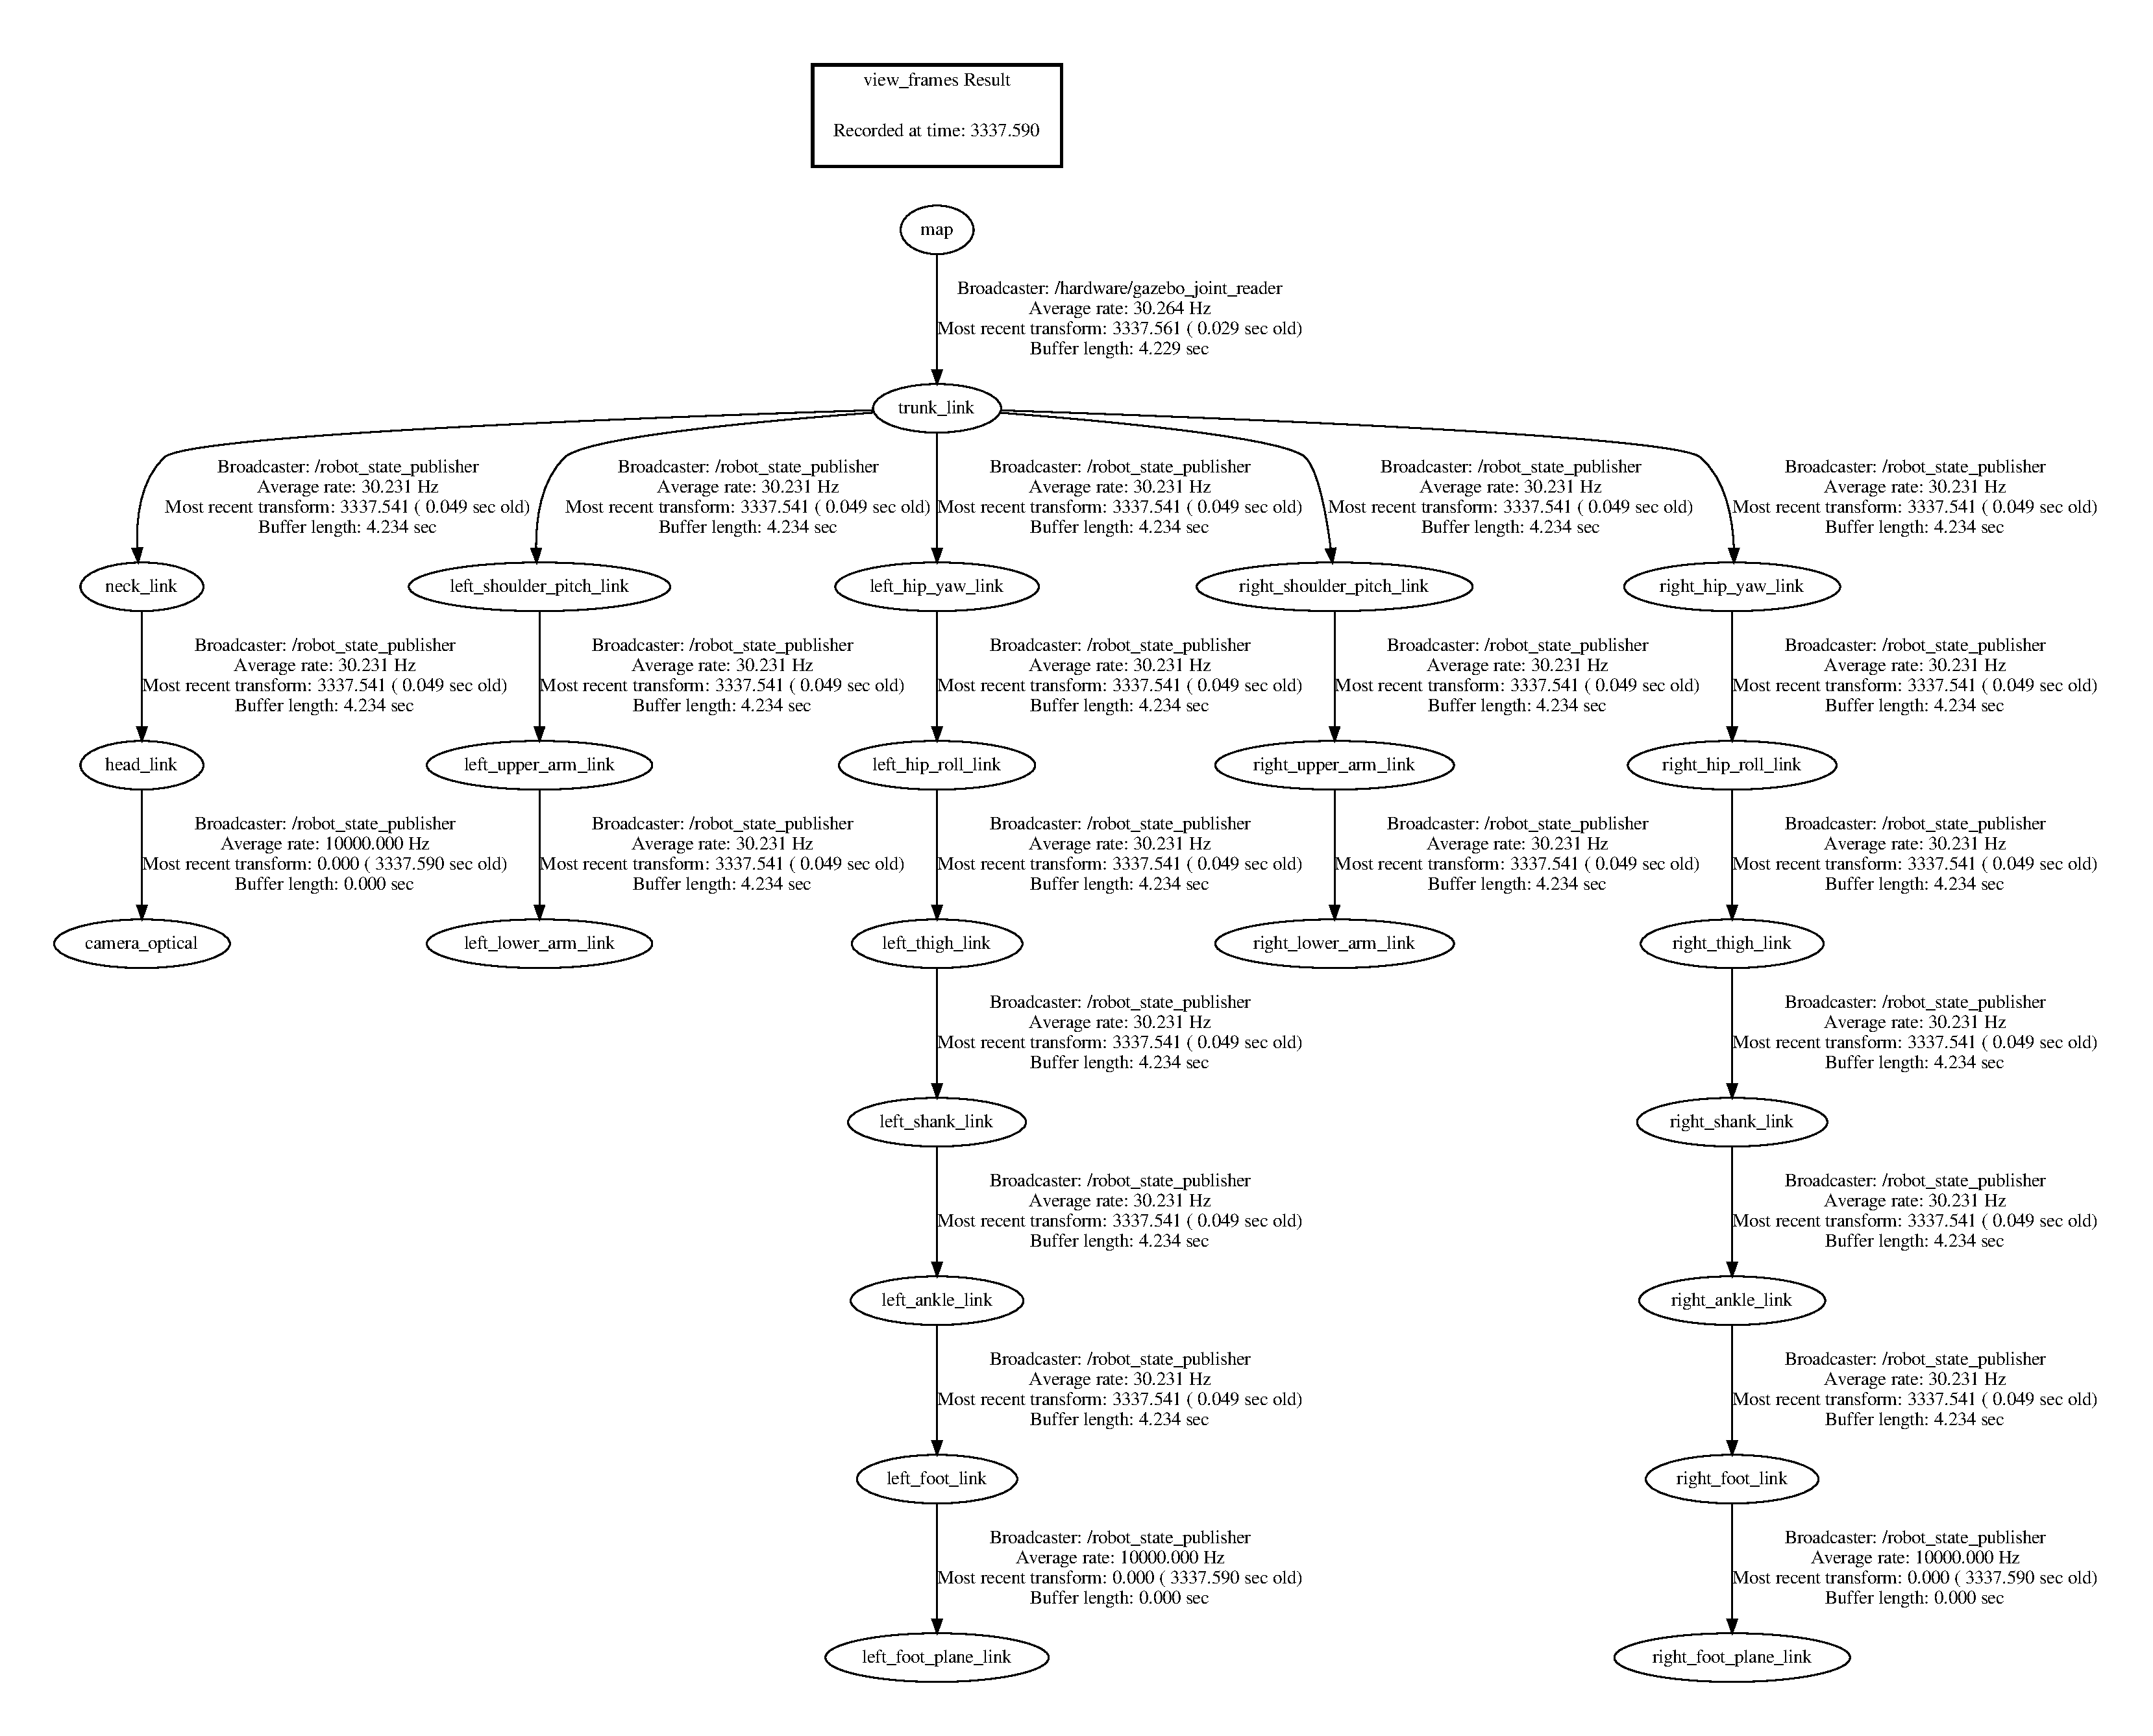
\includegraphics[width=\textwidth]{frames.pdf}
  \caption{Ejemplo del árbol de transformaciones del paquete \texttt{tf}.}
  \label{fig:frames}
\end{figure}

\subsection{El formato \textit{urdf}}

\section{Desarrollo}

\section{Evaluación}

\end{document}
